% To je predloga za poročila o domačih nalogah pri predmetih, katerih
% nosilec je Blaž Zupan. Seveda lahko tudi dodaš kakšen nov, zanimiv
% in uporaben element, ki ga v tej predlogi (še) ni. Več o LaTeX-u izveš na
% spletu, na primer na http://tobi.oetiker.ch/lshort/lshort.pdf.
%
% To predlogo lahko spremeniš v PDF dokument s pomočjo programa
% pdflatex, ki je del standardne instalacije LaTeX programov.

\documentclass[a4paper,11pt]{article}
\usepackage{a4wide}
\usepackage{fullpage}
\usepackage[utf8x]{inputenc}
\usepackage[slovene]{babel}
\selectlanguage{slovene}
\usepackage[toc,page]{appendix}
\usepackage[pdftex]{graphicx} % za slike
\usepackage{setspace}
\usepackage{color}
\definecolor{light-gray}{gray}{0.95}
\usepackage{listings} % za vključevanje kode
\usepackage{hyperref}
\renewcommand{\baselinestretch}{1.2} % za boljšo berljivost večji razmak
\renewcommand{\appendixpagename}{Priloge}

\lstset{ % nastavitve za izpis kode, sem lahko tudi kaj dodaš/spremeniš
language=Python,
basicstyle=\footnotesize,
basicstyle=\ttfamily\footnotesize\setstretch{1},
backgroundcolor=\color{light-gray},
}

\title{Nekaj lastnosti podatkov o razvrščanju člankov v tematske skupine}
\author{Gregor Majcen (63070199)}
\date{\today}

\begin{document}

\maketitle

\section{Uvod}
Prva domača naloga je namenjena, da se seznanimo s tipom podatkov, ki jih bomo tudi v nadalnje uporabljali in pa tudi malo o statistiki le teh. Odgovoriti je potrebno na 8 vprašanj, med katerimi so 3 lastna.

\section{Rezultati}

\begin{description}
\item[Koliko primerov vsebujejo podatki?] \hfill \\ 2000 primerov 
\item[Koliko atributov vsebujejo podatki?] \hfill \\ 10000 atributov
\item[Kakšnega tipa so atributi?] \hfill \\ zvezni
\item[Kakšen delež elementov matrike ima vrednost različno od 0?] \hfill \\ 0.412115\%
\item[Koliko je vseh različnih oznak (razredov) v podatkih?] \hfill \\ 82 različnih oznak
\item[Koliko neničelnih atributov ima primer, ki ima največ atributov enakih 0?] \hfill \\ 21 atributov  
\item[Koliko neničelnih atributov ima primer, ki ima največ atributov različnih od 0?] \hfill \\ 79 atributov
\item[Koliko je primerov, ki imajo manj kot 30 neničelnih atributov?] \hfill \\ 1878 primerov
\item[Koliko je atributov, ki imajo povsod vrednost enako 0?] \hfill \\ 2349 atributov

\item[Koliko atributov ima vrednost različno od 0 za posamezen primer?] \hfill \\
\begin{figure}[h!]
\begin{center}
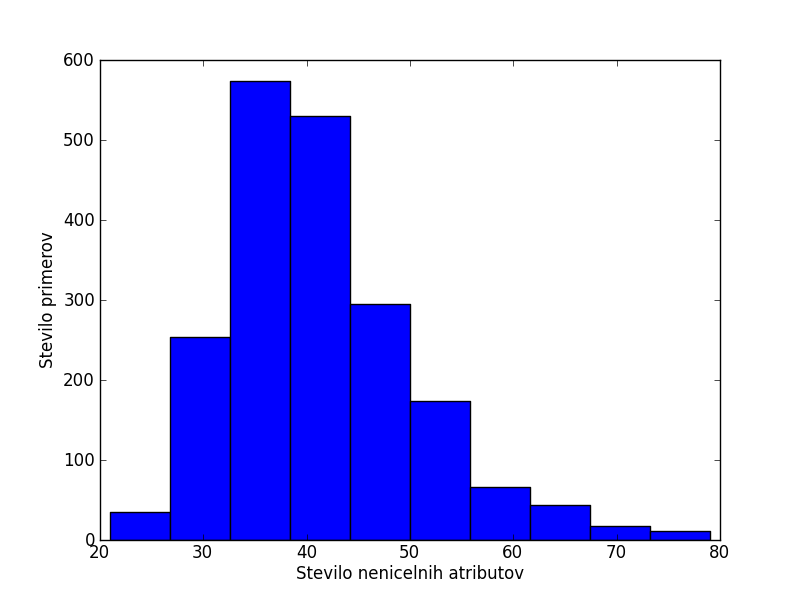
\includegraphics[scale=0.5]{statPrimeri.png}
\caption{Histogram, ki prikazuje koliko je neničelnih atributov za posamezen primer}
\label{slika1}
\end{center}
\end{figure}

Z grafa je lepo opazno, da je največ primerov s približno 35 do 45 neničelnimi atributi. 

\item[V koliko primerih atribut zavzame neničelne vrednosti?] \hfill \\
\begin{figure}[h!]
\begin{center}
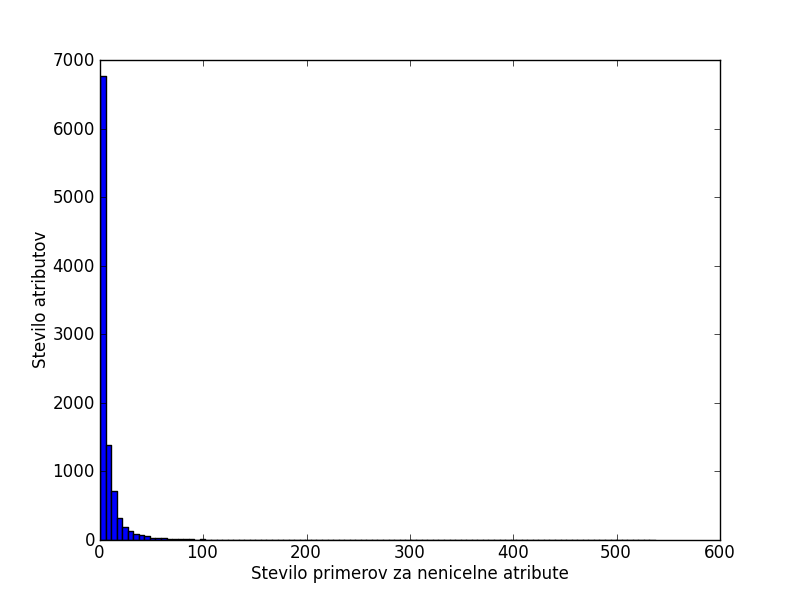
\includegraphics[scale=0.5]{statAttr.png}
\caption{Histogram, ki prikazuje v koliko primerih atribut zavzame neničelne vrednosti}
\label{slika2}
\end{center}
\end{figure}

Z grafa je lepo opazno, da je zelo malo izkoriščenih atributov, saj je vse zelo blizu ničle.

\pagebreak
\item[S koliko različnimi oznakami so označeni primeri?] \hfill \\
\begin{figure}[h!]
\begin{center}
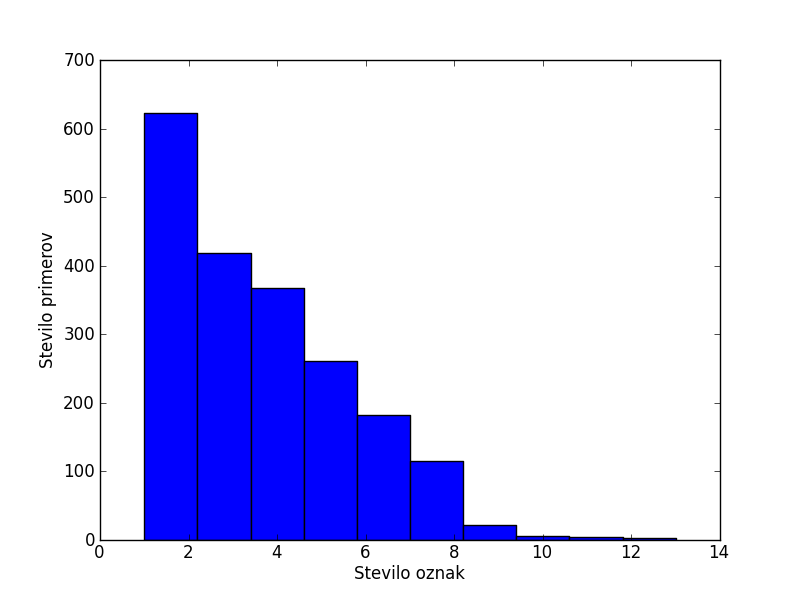
\includegraphics[scale=0.5]{statRazredi.png}
\caption{Histogram, ki prikazuje s koliko različnimi oznakami so označeni primeri}
\label{slika3}
\end{center}
\end{figure}

Z grafa je lepo opazno, da sta dve oznaki za primer kar najbolj pogosti, nato pa vseskozi manj pogosto. 

\end{description}

\pagebreak

\section{Izjava o izdelavi domače naloge}
Domačo nalogo in pripadajoče programe sem izdelal sam.

\end{document}
